\clearpage % clear the prior chapter's page

\chapter{\mytool: Usage, Architecture, and Implementation Details}\label{CH4_ToolUsage}
%\vspace{-7mm}
%\bigskip

\section{Usage}
For ease of this experiment, we have created a tool, \mytool~\cite{weber_2022}, that will simplify the unit tests. To use this tool, the developer will only have to provide the following: test file with full path, name of the test (as a single file can have many tests and we may want to reduce only one failing test), and the path of the \texttt{.csproj} file associated with the code. All of this information is already available to the developers. Optionally, the developer can provide a particular folder path if they want to use it to store intermediate results and the final output in that folder. An example of this execution can be seen in figure~\ref{fig:command}. The architecture from a developer's perspective is described in figure~\ref{fig:tool_architecture}. If you compare the architecture figure with the \emph{Perses} workflow figure and the \emph{Picireny} architecture figure, the contrast is clear~\cite{hodovan2016modernizing, perses}. Both the \emph{Perses} and \emph{Picireny} approaches require significant preprocessing steps that require other libraries, toolsets, and components. Both of them require a test script to be available, normally a shell file or a batch file. \mytool does not require any of these as explained in the architecture section. 

\begin{figure*}
\begin{lstlisting}
ReduSharptor.exe ".\language-ext\LanguageExt.Tests\ApplicativeTests.cs" "ListCombineTest" ".\language-ext\LanguageExt.Tests\LanguageExt.Tests.csproj" ".\Simplified Test Results"
\end{lstlisting}
\caption{\texttt command line execution of \mytool}
\label{fig:command}
%\vspace{-0.5in}
\end{figure*}

\begin{center}
\begin{figure}[!ht]
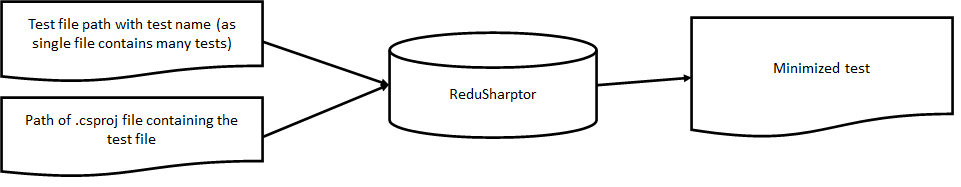
\includegraphics[width=\linewidth]{tool_archicture.png}
\caption{\mytool architecture from a user's perspective}
\label{fig:tool_architecture}
\end{figure}
\end{center}

\section{Architecture}
As \mytool is implemented for C\#, it takes into consideration how C\# programs are organized using \texttt{.sln} and \texttt{.csproj} files. In order to compile or run the test, \mytool uses the \texttt{.csproj} file, the test, and the built-in build+run utility available as part of the \texttt{.NET} framework and Roslyn compiler to generate the necessary build+run script. The process is described in the right side of figure~\ref{fig:internal}. On the left side, we describe how a test is processed first using the Roslyn compiler to generate the parse tree. The parse tree will go through a pruning and transformation process to produce a tree where \emph{Tree} statements will be processed as \emph{NonTree} statements. The test, the processing statement list, and the build+run script will then be passed to the DD algorithm to produce the minimized test. The \emph{Perses} and \emph{Picireny} approaches require the user of their tool to provide a test script which may increase in complexity over time as both approaches will require a new test script for each test minimization. 

\begin{center}
\begin{figure}[!ht]
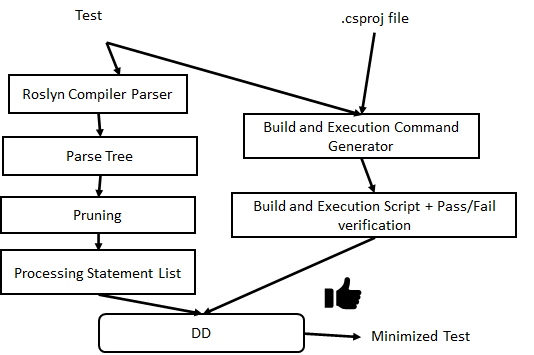
\includegraphics[width=\linewidth]{internal_architecture.png}
\caption{\mytool internal architecture with implementation details}
\label{fig:internal}
\end{figure}
\end{center}

In addition, a great effort was made to not have any external dependencies, libraries, or tool sets and, as a result, \mytool only utilizes the \texttt{.NET} framework and Roslyn compiler API, which is available as part of the \texttt{Microsoft.CodeAnalysis} library. Therefore, a user can easily invoke \mytool as a command line utility without the needing to download or maintain any external components or libraries. Because \mytool is a C\# specific tool designed for C\# unit tests, the need for preprocessing steps is eliminated.

\section{Implementation}

The execution of the simplification process is rather simple. It separates the tests into sections of statements and attempts to run each section as a standalone test. If any of the sections result in a failed test, that section is made the new test and the process is repeated. Otherwise, the complement of each section is attempted and, likewise, is made the new test if any of them fail. If none of the sections or their complements fail, then the granularity of the sections is increased and the process is repeated. This process is continued until all sections result in successful runs and the sections cannot be reduced any further. This is an adapted form of the work of A. Zeller et al.~\cite{zeller2002simplifying}. However, instead of using a set of failing input values, this approach simplifies and isolates the unit test statements themselves.

In \mytool, this primary simplification code exists within the \texttt{FindSmallestFailingInput} method from figure~\ref{fig:FindSmallestFailingInput1}. Each \texttt{foreach} block tests the sections and their complements and are then checked to see if any of the tests are successful. Following those blocks, the granularity of the sections is increased on line 51, then checked against the number of remaining statements to ensure the number of sections does not exceed the amount of statements. If the level of granularity if more than the remaining statements, then the simplification process is finished.

In order to understand the tool fully, a great understanding must be had about how these algorithms were originally implemented. In figure~\ref{fig:Main1} rests the \mytool entry point, the \texttt{Main} method. After taking input from the command line arguments, this gets the statements from the provided unit test and creates a copy as a backup. The \texttt{Main} method then calls \texttt{FindSmallestFailingInput}, which starts the simplification algorithm. After producing the simplified output, it reverts the test file to its original state and outputs the simplified statements into a separate file.

The Roslyn compiler is used in a few of the methods: figures~\ref{fig:GetTestStatements1}, \ref{fig:SetTestStatements1}, and \ref{fig:GetTestCallString1}. \texttt{GetTestStatements} and \texttt{SetTestStatements} both use Roslyn in similar ways to break apart the file and find the unit test from a name, however, \texttt{SetTestStatements} also uses Roslyn in order to write a new list of statements to the unit test. \texttt{GetTestCallString} is a little different as it is only used to create a string used to build the unit test for each compilation process. This is an additional performance increase that was utilized to speed up the process.

In figure~\ref{fig:BuildAndRunTest1}, the \texttt{BuildAndRunTest} method is relatively straightforward; it first builds and then runs the test. If the test passes, it will return \texttt{true} for the \texttt{FindSmallestFailingInput} test to be used in that algorithm. However, one piece of logic needs clarification: if the test fails to build, we return \texttt{true}. Returning a \texttt{true} value will notify the algorithm to continue with the process. Additionally, \texttt{BuildAndRunTest} is passed to the \texttt{FindSmallestFailingInput} method as an action to call. This will allow the algorithm to test each variant with this method. 

In correspondance with the previously mentioned methods, figures ~\ref{fig:GetDividedSections1}, ~\ref{fig:GetSectionCompliment1}, ~\ref{fig:WaitForFile1}, and ~\ref{fig:ExecuteCommand1} are also included. These are used to reduce the amount of code, and allow for an easy interpretation.
